%%%%%%%% MLSys 2024 FINAL REPORT %%%%%%%%%%%%%%%%%

\documentclass{article}

\usepackage{microtype}
\usepackage{graphicx}
\usepackage{subfigure}
\usepackage{booktabs}
\usepackage{hyperref}
\usepackage{algorithm}
\usepackage{algorithmic}
\usepackage{amsmath}
\usepackage{multirow}
\usepackage{xcolor}
\usepackage{listings}
\usepackage{enumitem}
\usepackage{titlesec}
\usepackage{float}  % Provides [H] strict-here float placement for appendix tables

\usepackage[accepted]{mlsys2024}

% --- Replace mlsys2024's \@makecaption with tighter spacing:
%     6pt (was 10pt) before caption, 6pt (was 0pt) after caption.
%     Must use \AtBeginDocument because mlsys2024 defines its own version
%     that would otherwise override ours. \makeatletter MUST be outside the
%     \AtBeginDocument hook (otherwise @ is "other" when the token list is
%     parsed, and \@makecaption gets mis-tokenized).
\makeatletter
\AtBeginDocument{%
  \long\def\@makecaption#1#2{%
    \vskip 6pt
    \baselineskip 11pt
    \setbox\@tempboxa\hbox{#1. #2}%
    \ifdim \wd\@tempboxa >\hsize
      \sbox{\newcaptionbox}{\small\sl #1.~}%
      \newcaptionboxwid=\wd\newcaptionbox
      \usebox\newcaptionbox {\footnotesize #2}%
    \else
      \centerline{{\small\sl #1.} {\small #2}}%
    \fi
    \vskip 6pt}%
}
\makeatother

% --- Global compact list spacing ---
\setlist[itemize]{itemsep=2pt,topsep=3pt,parsep=1pt,partopsep=0pt,leftmargin=*}
\setlist[enumerate]{itemsep=2pt,topsep=3pt,parsep=1pt,partopsep=0pt,leftmargin=*}

% --- Compact \paragraph spacing ---
\titlespacing*{\paragraph}{0pt}{0.4em}{0.5em}

% --- Be more permissive about float placement to avoid bottom whitespace ---
\renewcommand{\topfraction}{0.95}
\renewcommand{\bottomfraction}{0.85}
\renewcommand{\textfraction}{0.05}
\renewcommand{\floatpagefraction}{0.85}

% --- Avoid stretching vertical glue (default \flushbottom in two-column
%     produces visible whitespace between paragraphs and around floats)
\raggedbottom

% --- Python code listing style for Implementation Details ---
\definecolor{codekw}{RGB}{0,0,180}
\definecolor{codestr}{RGB}{163,21,21}
\definecolor{codecmt}{RGB}{0,128,0}
\definecolor{codebg}{RGB}{248,248,248}
\lstdefinestyle{pystyle}{
  language=Python,
  basicstyle=\scriptsize\ttfamily,
  keywordstyle=\color{codekw}\bfseries,
  stringstyle=\color{codestr},
  commentstyle=\color{codecmt}\itshape,
  backgroundcolor=\color{codebg},
  showstringspaces=false,
  numbers=none,
  frame=single,
  framerule=0.3pt,
  rulecolor=\color{black!30},
  xleftmargin=4pt,
  xrightmargin=4pt,
  aboveskip=4pt,
  belowskip=4pt,
  columns=fullflexible,
  breaklines=true,
  keepspaces=true,
}
\lstset{style=pystyle}

\mlsystitlerunning{RAGCache++: Cache-Aware Document Ordering for Low-Latency RAG Serving}

\begin{document}

\twocolumn[
\mlsystitle{RAGCache++: Cache-Aware Document Ordering\\for Low-Latency RAG Serving}

\mlsyssetsymbol{equal}{*}

\begin{mlsysauthorlist}
\mlsysauthor{Kaizhen Tan}{equal,cmu}
\mlsysauthor{Rong Gu}{equal,cmu}
\mlsysauthor{Mingyuan Li}{equal,cmu}
\end{mlsysauthorlist}

\mlsysaffiliation{cmu}{Heinz College of Information Systems and Public Policy, Carnegie Mellon University, Pittsburgh, PA, USA}

\mlsyscorrespondingauthor{Kaizhen Tan}{kaizhent@cmu.edu}
\mlsyscorrespondingauthor{Rong Gu}{ronggu@andrew.cmu.edu}
\mlsyscorrespondingauthor{Mingyuan Li}{mingyua4@andrew.cmu.edu}

\mlsyskeywords{RAG, LLM Serving, KV Cache, Prefix Caching, Latency Optimization}

\vskip 0.3in

\begin{abstract}
Retrieval-Augmented Generation (RAG) improves factual grounding, but it also makes prompts much longer and increases prefill latency. Prefix caching in modern serving engines such as vLLM can reduce this cost, but it only works when different requests share the same token prefix. In practice, RAG queries often retrieve overlapping documents in different orders, so document overlap does not automatically become prefix overlap. We present RAGCache++, a lightweight prompt-layer method that reorders retrieved documents before inference. The method keeps a prefix tree over recently served document sequences and uses a greedy walk to place the most reusable prefix first, while leaving the serving engine unchanged. Across two vLLM configurations, our method reduces median TTFT by about 20\%--33\% compared with retrieval-order prefix caching, without hurting answer quality in our QA tests. We further show that the greedy policy reaches 97.5\% of oracle ordering gain, suggesting that most reusable prefix locality can already be recovered with a simple scheduling layer between retrieval and serving. 
\end{abstract}
]

\printAffiliationsAndNotice{\mlsysEqualContribution}


% ================================================================
\section{Introduction and Motivation}
\label{sec:intro}
% ================================================================

Retrieval-Augmented Generation (RAG) improves factual grounding by adding external passages to the prompt before generation~\citep{lewis2020rag,gao2024ragsurvey}. The price is higher serving latency. In many RAG systems, the retrieved context dominates the input length, so the prefill stage becomes the main bottleneck for interactive use.

Modern serving engines partly address this problem with prefix caching. Serving systems such as vLLM and SGLang can reuse previously computed KV states through Automatic Prefix Caching (APC) when a new request shares the same token prefix with an earlier one~\citep{vllm_apc,zheng2024sglang}. This mechanism works well for highly repetitive prompts, but it is much less effective in RAG, where retrieved passages may overlap in content while appearing in different orders.

This mismatch is the central problem of this paper. Prefix caching works at the token level, while retrieval returns documents at the chunk level. Two consecutive queries may retrieve almost the same evidence set, but once the first document differs, the shared token prefix is broken and most reusable KV blocks are lost. In other words, document overlap is common in RAG, but prefix overlap is much rarer.

Our key idea is simple: instead of changing the serving engine, change the document order before the prompt is built. If retrieved documents are reordered to follow a recently cached sequence, the resulting prompt is more likely to match an existing prefix and benefit from APC. Based on this idea, we propose RAGCache++, a lightweight prompt-layer scheduler. It maintains a knowledge tree over recently served document sequences and uses a greedy walk to place the longest likely cached prefix first. The remaining documents are appended in retrieval order, so the system still falls back to the original ranking when reuse is unavailable.

Recent systems have shown that context order can affect cache reuse in long-context and RAG serving~\citep{jin2025ragcache,cachecraft2025,contextpilot2025}. Our goal is therefore not to re-establish that ordering matters, but to ask how much of this benefit can already be recovered with a minimal and engine-agnostic design. In our setting, the core policy stays entirely at the prompt-construction layer, requires no modification to vLLM, and still performs close to exhaustive oracle ordering in our evaluation.

This paper studies three questions. First, can a pure prompt-layer policy provide meaningful TTFT gains in APC-based RAG serving? Second, is a greedy trie traversal sufficient, or does the problem require substantially more complex search? Third, do the gains remain visible beyond a single synthetic benchmark, under different overlap levels, workloads, and concurrent execution settings? Our results indicate that the answer is yes in all three cases.


\section{Related Work and Background}
\label{sec:background}
% ================================================================

\subsection{RAG Serving Pipeline}

A standard RAG pipeline has four steps: query encoding, document retrieval, prompt construction, and LLM inference. In practice, prompt construction is cheap, while inference dominates latency. For this reason, the main serving problem is not how to concatenate the retrieved passages, but how to reduce repeated prefill work when many requests contain overlapping context.

\subsection{vLLM Automatic Prefix Caching}

vLLM manages KV cache memory in fixed-size blocks through PagedAttention~\citep{kwon2023pagedattention} and provides Automatic Prefix Caching (APC) on top of this design~\citep{vllm_apc}. APC reuses cached KV blocks when a new request shares the same token prefix as an earlier one. The design documentation further explains that vLLM hashes each block together with its prefix history, so reuse is inherently prefix-sensitive.

This detail matters for RAG. Once an early block differs, the later blocks no longer line up with the cached chain, even if the two prompts still contain many of the same documents. Therefore, a small difference near the beginning of the prompt can remove most of the possible reuse.

\textbf{Implication for RAG.} In document retrieval, overlap is usually set-based, while APC requires ordered prefix agreement. If two requests retrieve the same documents in different positions, their token prefixes diverge immediately and reuse drops sharply. Figure~\ref{fig:prefix_blocks} illustrates this gap and shows why reordering is a natural intervention point.

\begin{figure}[t]
\centering
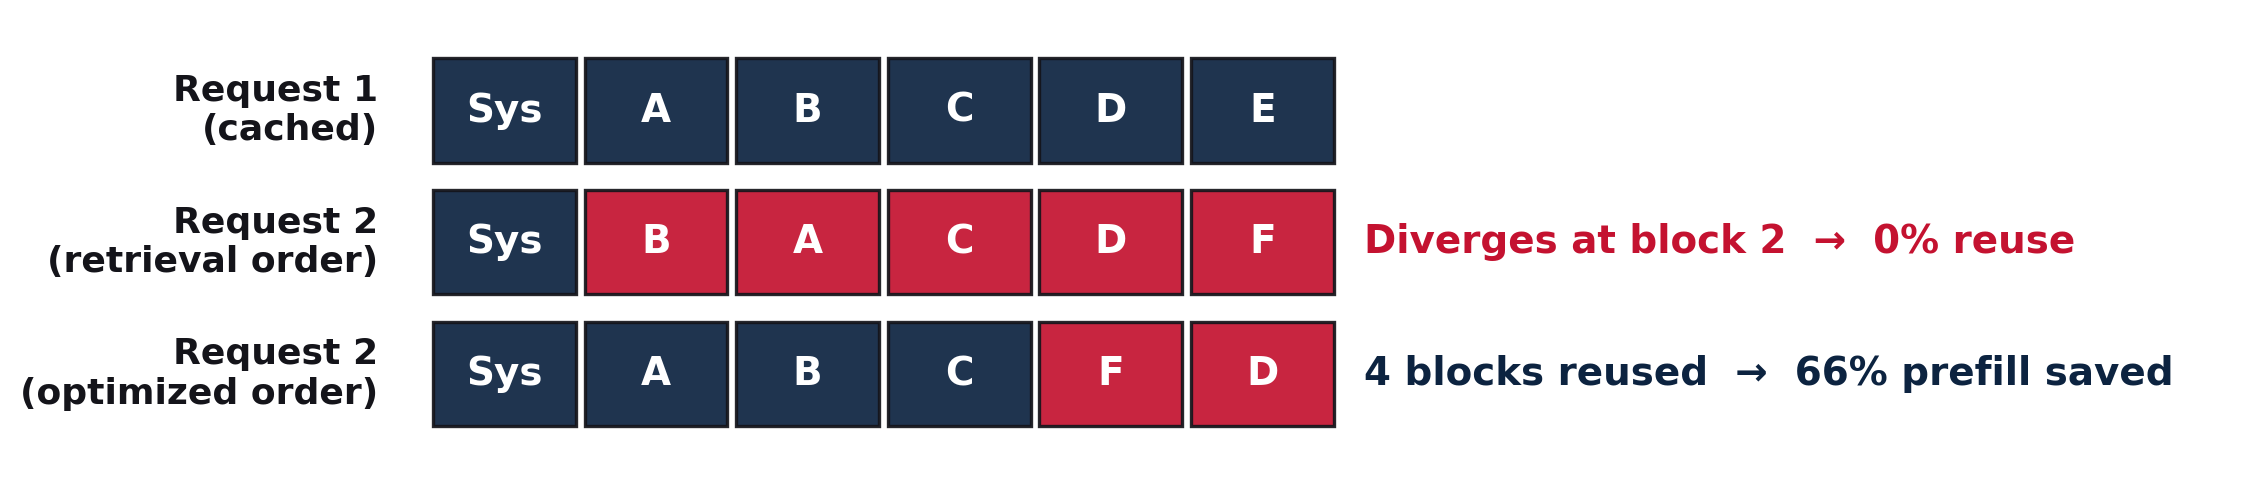
\includegraphics[width=\linewidth]{figures/prefix_blocks.png}
\caption{Prefix alignment in APC-based RAG serving. Request~1 is cached. Request~2 shares 60\% of its documents but in retrieval order the prefix diverges at block~2, yielding 0\% reuse. Reordering the shared documents to the front restores prefix alignment: 4 blocks reused, 66\% prefill saved.}
\label{fig:prefix_blocks}
\vspace{-1em}
\end{figure}

\subsection{Related Work}

Several recent papers study KV reuse in long-context or RAG inference, but they do so at different layers of the system.

\textbf{RAGCache}~\citep{jin2025ragcache} is the closest work to ours. It also uses a tree structure over document sequences, but its design is tied to a richer cache-management stack inside the serving system. Our work borrows the basic intuition of sequence-aware reuse, but focuses on a smaller target: document ordering at the prompt layer, with no engine modification.

\textbf{ContextPilot}~\citep{contextpilot2025} studies context reuse for long-context inference and proposes a context index, context ordering, and de-duplication. Its results support the same broader message as ours: prefill can often be reduced by reorganizing context before inference, rather than by redesigning the model itself.

\textbf{Cache-Craft}~\citep{cachecraft2025} shows that plain prefix caching can be weak in production RAG workloads because retrieved chunks and their relative order vary across requests. This directly motivates our setting. Instead of replacing prefix caching, we try to make more requests compatible with it.

\textbf{TurboRAG}~\citep{turborag2024} and \textbf{CacheBlend}~\citep{yao2025cacheblend} address a harder problem: KV reuse even when reusable chunks are not part of one contiguous prefix. These approaches are more general than ours, but also more involved. Our method is narrower, but it is easy to deploy because it works with existing APC mechanisms.

\textbf{CacheGen}~\citep{lmcache2024} focuses on compressing and streaming KV caches efficiently. This is orthogonal to our setting. In principle, cache compression and cache-aware ordering could be combined in one serving stack.


\section{Methodology}
\label{sec:design}
% ================================================================

\subsection{Overview}

RAGCache++ sits between retrieval and prompt construction. Given a retrieved document set, it reorders the documents so that the final prompt is more likely to share a long prefix with recently served prompts. The serving engine still performs all KV-cache allocation and reuse; our layer only decides the document order.

\subsection{Knowledge Tree}

The knowledge tree is a trie whose root-to-leaf paths record document orders that have recently appeared in served requests. Each node stores a document ID together with lightweight metadata about recent use.

The tree supports two basic operations. First, after a request finishes, its ordered document sequence is inserted into the trie. Second, when a new request arrives, the trie is consulted to estimate which document order is most likely to align with a cached prefix. The tree therefore acts as a compact memory of recent prompt structure, rather than as a replacement for vLLM's own KV cache.

\subsection{Greedy Ordering Algorithm}

Our ordering policy is shown in Algorithm~\ref{alg:ordering}. Starting from the trie root, the algorithm repeatedly asks whether one of the remaining retrieved documents extends a cached path. If yes, that document is placed next in the prompt. If no cached continuation exists, the remaining documents are appended in their original retrieval order.

\begin{algorithm}[t]
\caption{Cache-aware document ordering}
\label{alg:ordering}
\begin{algorithmic}[1]
\REQUIRE Retrieved doc IDs $D = \{d_1, \ldots, d_k\}$ (in retrieval rank), knowledge tree $T$
\ENSURE Ordered sequence $O$
\STATE $O \leftarrow []$, $R \leftarrow D$, $\textit{node} \leftarrow T.\text{root}$
\WHILE{$R \neq \emptyset$}
    \STATE $\textit{found} \leftarrow \texttt{false}$
    \FOR{each $d \in R$}
        \STATE $c \leftarrow \textit{node}.\text{getChild}(d)$
        \IF{$c \neq \texttt{null}$ \AND $c.\text{isCached}()$}
            \STATE Append $d$ to $O$; remove $d$ from $R$
            \STATE $\textit{node} \leftarrow c$; $\textit{found} \leftarrow \texttt{true}$; \textbf{break}
        \ENDIF
    \ENDFOR
    \IF{$\textit{found} = \texttt{false}$}
        \STATE Append remaining $R$ in retrieval-rank order to $O$
        \STATE \textbf{break}
    \ENDIF
\ENDWHILE
\STATE \textbf{return} $O$
\end{algorithmic}
\end{algorithm}

This policy is intentionally simple. It does not try to solve a full combinatorial search problem at runtime. Instead, it greedily extends the longest usable prefix it can find from the current trie state. Figure~\ref{fig:trie} shows the intuition.

\begin{figure}[t]
\centering
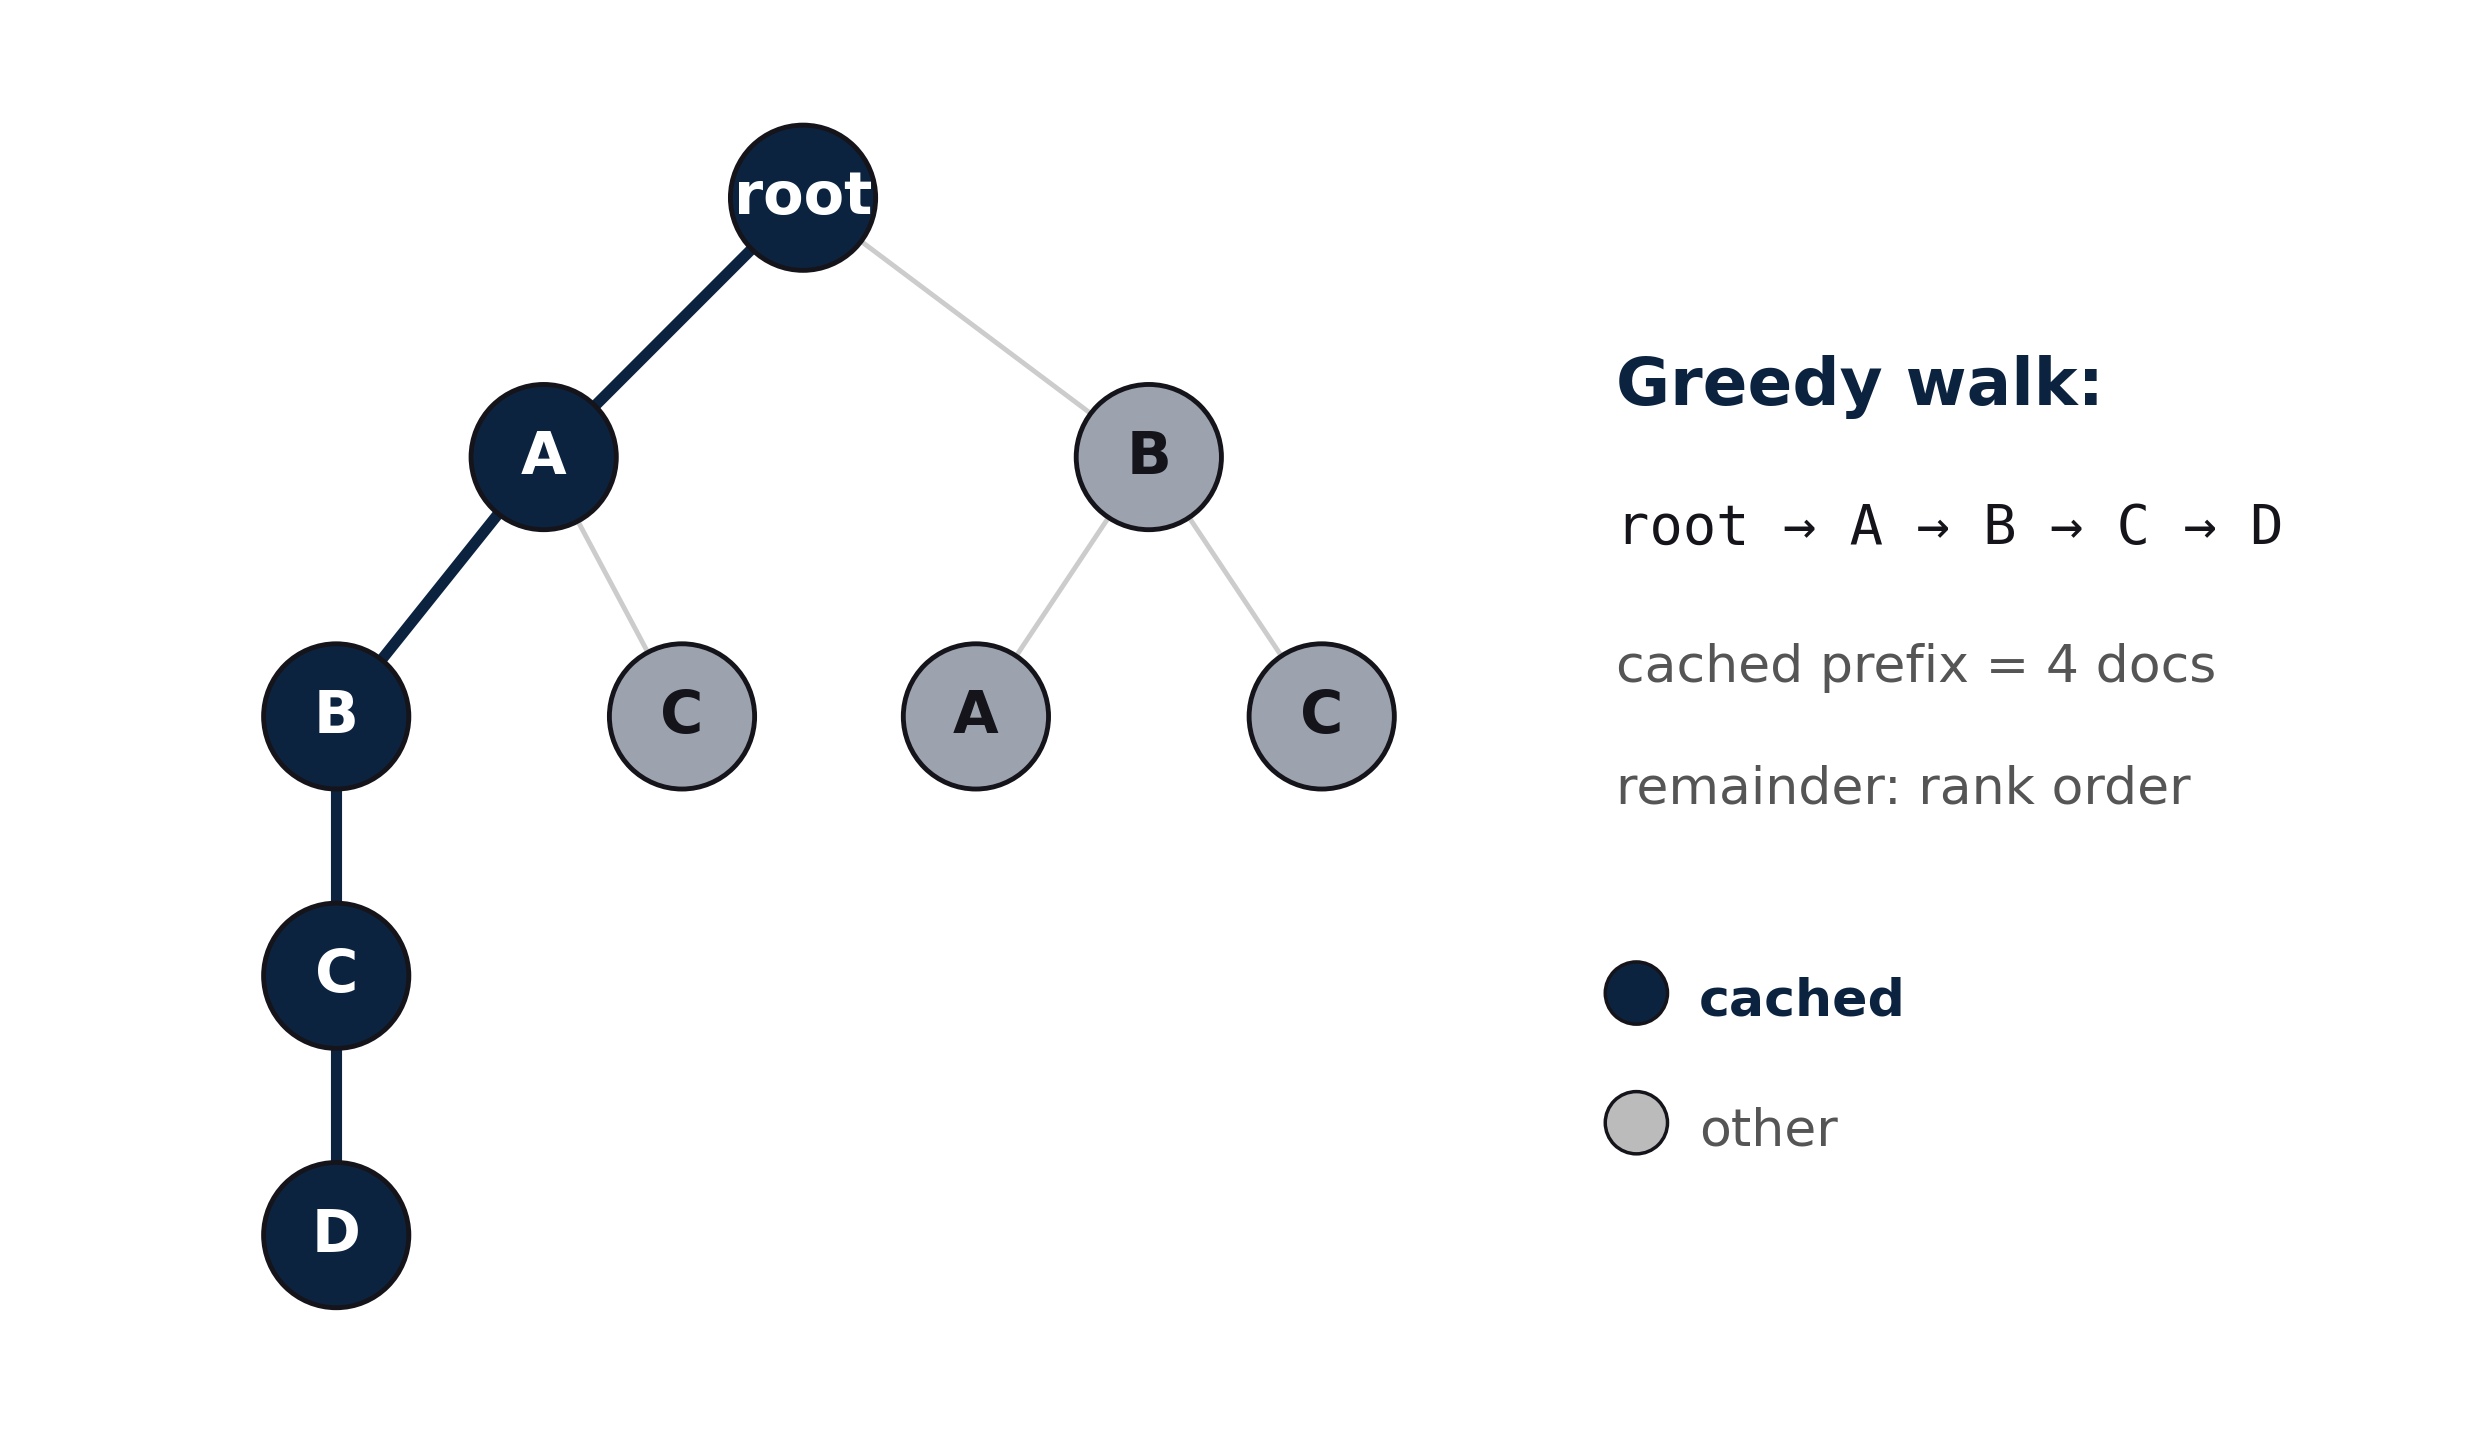
\includegraphics[width=\linewidth]{figures/trie_diagram.png}
\caption{Knowledge tree example. Dark nodes are cached; gray nodes are evicted or from other branches. Given candidate set $\{A,B,C,F,D\}$, the greedy walk follows root$\to$A$\to$B$\to$C$\to$D (the longest cached path), yielding a 4-document prefix hit. The remaining document (F) is appended in retrieval-rank order.}
\label{fig:trie}
\vspace{-1em}
\end{figure}

The objective behind this policy is straightforward. APC benefits grow with the length of the shared prefix, so we want the reordered prompt to match as many leading documents of a cached sequence as possible. The greedy walk is inexpensive for typical top-$k$ values, and our later experiments show that it is already very close to oracle ordering.

\subsection{Knowledge Tree as an Approximate Cache Index}

The knowledge tree is only an approximation of the actual APC state. It records what has been served recently, not what remains resident in GPU memory. This distinction matters because vLLM controls block eviction internally. As a result, the trie can sometimes predict reuse for a path whose KV blocks have already been evicted.

We treat this mismatch as a systems issue rather than a modeling failure. In stable sequential runs, the approximation is often good enough by itself. Under tighter memory or more concurrent execution, we add a lightweight feedback mechanism to detect stale paths and prune them.

\subsection{Integration with vLLM}

The integration with vLLM has three pieces: a prompt builder that accepts retrieved documents and applies the ordering policy, a knowledge tree maintained at the application layer, and ordinary \texttt{LLM.generate()} calls with APC enabled. No internal vLLM symbols are required. This is important for portability, because it keeps the method close to a drop-in middleware component rather than a custom fork of the serving engine.

\subsection{Cache-State Feedback Loop}
\label{sec:feedback}

To reduce trie staleness, we use a TTFT-based feedback loop. The intuition is that if the trie predicts a long reusable prefix but the observed TTFT is still close to a cold request, then the supposed cached path is probably no longer resident. In that case, we mark the path as stale and stop relying on it.

This feedback loop closes the gap between logical reuse and physical cache residency. The trie proposes a likely reusable ordering, vLLM executes the request, and the observed TTFT is used to decide whether the trie should trust that path in the future. The mechanism is simple, but it lets the prompt-layer policy adapt online without direct instrumentation of vLLM internals.

\subsection{Retrieval-Inference Pipelining}

Besides document ordering, we also implement a secondary optimization that overlaps retrieval with a small warmup request. The system prompt is identical across requests, so its KV states can be prefetched while the retriever is still working. When retrieval finishes, the full request can reuse this shared prefix immediately.

This pipelining idea is orthogonal to our main contribution. It does not change the ordering policy, and it mainly helps cold starts or recovery after eviction. We include it because it fits the same design philosophy: reduce prefill waste without changing the serving engine itself.


\section{Implementation Details and Code Snippets}
\label{sec:impl}
% ================================================================

RAGCache++ is implemented as a Python package on top of vLLM and FastAPI. The implementation has two layers. The first is the minimal ordering path, which contains the trie walk and prompt construction logic used in the main experiments. The second is a fuller proxy system that adds cache-state bookkeeping, feedback, and service integration. This split is useful in practice, because it separates the core idea from the engineering needed for a more complete serving prototype.

\subsection{Module Organization}

Table~\ref{tab:modules} summarizes the main modules. The cache-related components and the prompt builder are decoupled, so the ordering logic can be tested without running the full GPU serving stack.

\begin{table}[h]
\caption{Core-library modules (excludes benchmark scripts, workload generators, and evaluation harnesses). Cache subsystem and integration layer are decoupled: the trie + prompt builder can run without GPU for unit tests.}
\label{tab:modules}
\centering
\scriptsize
\resizebox{\columnwidth}{!}{%
\begin{tabular}{@{}lll@{}}
\toprule
\textbf{Module} & \textbf{LOC} & \textbf{Role} \\
\midrule
\texttt{cache/knowledge\_tree.py}      & 232 & Trie + KV metadata \\
\texttt{cache/cache\_manager.py}       & 615 & Multi-tier accounting \\
\texttt{cache/pgdsf\_policy.py}        & 153 & PGDSF eviction \\
\texttt{cache/spatial\_index.py}       & 317 & Geohash spatial filter \\
\texttt{vllm\_integration/prompt\_builder.py} & 107 & Greedy ordering + prompt \\
\texttt{vllm\_integration/serving.py}  & 296 & Proxy + feedback + API \\
\texttt{serving/rag\_controller.py}    & 361 & Pipelining controller \\
\texttt{config.py}                     & 102 & Config dataclasses \\
\bottomrule
\end{tabular}%
}
\vspace{-0.5em}
\end{table}

\subsection{Key Code Snippets}

\paragraph{Greedy trie-based ordering.} The policy itself is small. It walks the knowledge tree, extends a reusable prefix when possible, and otherwise falls back to retrieval order.

\begin{lstlisting}[caption={Greedy ordering (\texttt{prompt\_builder.py}). \texttt{remaining} is a \texttt{set}; when multiple cached children exist at one trie level the iteration order is Python-hash-dependent (ties are rare in practice---the trie typically has one matching child per level). The cold-path loop appends every remaining document in retrieval-rank order (matching Algorithm~\ref{alg:ordering}).},label={lst:order}]
def optimize_doc_order(doc_ids, kt):
    ordered, remaining = [], set(doc_ids)
    node = kt.root
    while remaining:
        found = False
        # Hot path: extend the cached prefix by one cached child
        for d in list(remaining):  # set order; tie-break is hash-dependent
            child = node.get_child(d)
            if (child is not None
                and child.kv_metadata is not None
                and child.kv_metadata.tier != "none"):
                ordered.append(d); remaining.discard(d)
                node = child; found = True
                break   # only break the inner for; outer while continues
        if not found:
            # Cold path: append ALL remaining docs in retrieval-rank
            # order, then exit the outer while loop.
            for d in doc_ids:
                if d in remaining:
                    ordered.append(d)
            break
    return ordered
\end{lstlisting}

\paragraph{TTFT-based mismatch detection.} Because the trie only approximates the actual cache state, the system uses TTFT observations to detect stale paths and prune them when needed.

\begin{lstlisting}[caption={Cache-state feedback (\texttt{serving.py}).},label={lst:feedback}]
def check_mismatch(self, predicted_prefix_len, k, ttft_ms):
    self.total_observations += 1
    pred_reuse   = predicted_prefix_len / max(k, 1)
    actual_reuse = max(0.0, 1.0 - ttft_ms / max(self.cold_ttft, 1.0))
    self.history.append((pred_reuse, actual_reuse))
    if pred_reuse > 0.3 and actual_reuse < 0.15:
        self.mismatches += 1
        return True              # trie thinks hit, vLLM evicted
    return False
\end{lstlisting}

\paragraph{Integrated serve loop.} In the full proxy, ordering, prompt build, inference, feedback, and admission are connected in a single request path.

\begin{lstlisting}[caption={\texttt{VLLMCacheProxy.serve\_request} (abridged).},label={lst:serve}]
def serve_request(self, query, doc_ids, doc_contents, max_tokens=1):
    # 1. Greedy trie walk -> ordered ids + predicted prefix length
    ordered, predicted = self._greedy_walk(doc_ids)
    # 2. Build prompt
    prompt, _ = build_rag_prompt(query, ordered, doc_contents)
    # 3. vLLM inference (APC enabled at LLM construction)
    t0 = time.perf_counter()
    out = self.llm.generate([prompt], sp)
    ttft_ms = (time.perf_counter() - t0) * 1000
    # 4. Feedback loop
    self.feedback.update_cold_estimate(ttft_ms, predicted, len(doc_ids))
    miss = self.feedback.check_mismatch(predicted, len(doc_ids), ttft_ms)
    # 5. Prune stale paths if vLLM evicted them
    if miss:
        self._prune_path(ordered[:predicted])
    # 6. Admit into multi-tier cache state
    metas = [self.cache_manager.admit(d, 200, retrieval_rank=i+1)
             for i, d in enumerate(ordered)]
    self.cache_manager.insert_sequence(ordered, metas)
    self.cache_manager.step()
    return {"ttft_ms": ttft_ms, "predicted_prefix_len": predicted, ...}
\end{lstlisting}

The practical point is that the optimization does not require deep changes to the serving engine. Existing RAG applications can adopt the method by adding a thin middleware layer around the standard inference call.

\subsection{Engineering Details and Trade-offs}

Several engineering choices are worth noting. First, we use the public vLLM API rather than private engine internals, which makes the integration easier to maintain across versions. Second, the fallback behavior is simple and safe: if the trie is empty or no cached continuation is found, the system returns to retrieval order. Third, the host-side data structure is lightweight, so the method does not trade lower TTFT for a large memory footprint outside the GPU.

Overall, the implementation reflects the same design goal as the method itself: keep the core mechanism small, keep the deployment path simple, and let the serving engine continue to handle actual KV management.


\section{Experiments}
\label{sec:eval}
% ================================================================

\subsection{Experimental Setup}

\textbf{Hardware.} We evaluate on two vLLM configurations: a smaller setup on RTX 4060~Ti with Qwen2.5-1.5B-Instruct, and a larger setup on RTX 4090 with Qwen2.5-7B-Instruct~\citep{qwen25tr}. Full software and hardware details are listed in Appendix~\ref{app:config}.

\textbf{Workload.} Our main benchmark uses a controlled synthetic corpus where consecutive queries within a burst retrieve overlapping documents. This setup is intentionally simple. It isolates the systems question of interest: when document overlap exists, can reordering turn that overlap into APC-friendly prefix reuse?

\textbf{Strategies.} We compare four settings: no cache, APC with retrieval order, APC with lexicographic sorting, and APC with our optimized ordering. Each setting is run with a fresh model instance to avoid contamination from previous cache state.

\textbf{Metrics.} We focus on TTFT, since document ordering mainly affects prefill rather than decode. We also report a cache-hit proxy, but we treat TTFT as the primary metric because it reflects both how often reuse happens and how deep the reusable prefix is.


\subsection{Main Results}

Table~\ref{tab:main} and Figure~\ref{fig:ttft} show the main result: optimized ordering consistently lowers median TTFT on both hardware configurations.

\begin{table}[t]
\caption{TTFT comparison across strategies and hardware. Best APC result in \textbf{bold}.}
\label{tab:main}
\centering
\small
\begin{tabular}{@{}llcccc@{}}
\toprule
\textbf{GPU} & \textbf{Strategy} & \textbf{p50} & \textbf{p95} & \textbf{Mean} & \textbf{Fast\%$^\dagger$} \\
\midrule
\multirow{4}{*}{\rotatebox{90}{\scriptsize 4060\,Ti}}
 & No Cache      & 158.2 & 161.4 & 158.3 & 0.0 \\
 & APC+Retrieval & 72.5  & 159.9 & 69.9  & 17.9 \\
 & APC+Sorted    & 108.0 & 164.9 & 101.7 & 25.3 \\
 & \textbf{APC+Optimized} & \textbf{57.9} & \textbf{161.3} & \textbf{68.1} & 18.9 \\
\midrule
\multirow{4}{*}{\rotatebox{90}{\scriptsize 4090}}
 & No Cache      & 121.3 & 123.7 & 121.4 & 0.0 \\
 & APC+Retrieval & 59.6  & 117.4 & 55.9  & 12.3 \\
 & APC+Sorted    & 81.2  & 118.7 & 76.3  & 25.6 \\
 & \textbf{APC+Optimized} & \textbf{40.1} & \textbf{117.4} & \textbf{51.4} & 19.0 \\
\bottomrule
\end{tabular}
\vspace{-0.5em}
\end{table}

\begin{figure}[t]
\centering
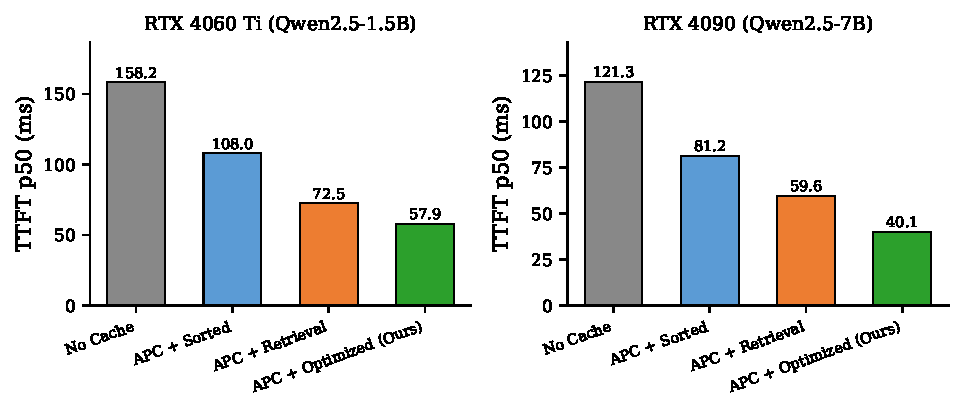
\includegraphics[width=\linewidth]{figures/ttft_comparison.pdf}
\caption{TTFT p50 comparison across strategies. Optimized ordering achieves the lowest latency on both GPUs despite not having the highest Fast\%$^\dagger$ proxy.}
\label{fig:ttft}
\vspace{-1em}
\end{figure}

Two observations are more important than the raw numbers. First, the gain is concentrated at p50 rather than p95. This is expected, because tail cases are often cold requests where no ordering policy can create reuse. Second, our method beats simple sorting even though sorting can show a higher hit-rate proxy. This tells us that not all hits are equally useful. A few long prefix matches matter more than many shallow ones.

\paragraph{Hit rate vs.\ latency.}

Figure~\ref{fig:hitrate} makes this point more clearly. The sorted baseline creates more fragmented matches, while our policy tries to preserve deeper contiguous prefixes. For APC-based serving, deeper reuse is the more valuable resource.

\begin{figure}[t]
\centering
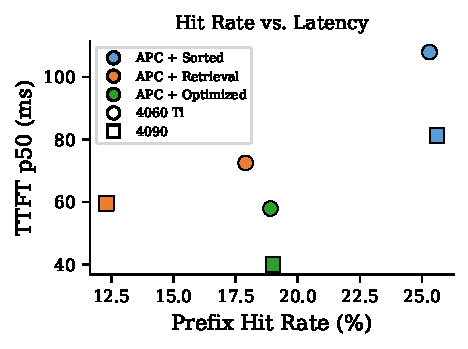
\includegraphics[width=0.85\linewidth]{figures/hitrate_vs_ttft.pdf}
\caption{Fast\%$^\dagger$ cache-hit proxy vs.\ TTFT across strategies and GPUs. A higher proxy value does not guarantee lower latency---prefix \emph{length} matters more than hit \emph{count}.}
\label{fig:hitrate}
\vspace{-1em}
\end{figure}



\section{Analysis, Ablations, and Findings}
\label{sec:analysis}
% ================================================================

\subsection{Overlap Sensitivity}

We next vary the amount of document overlap in the trace. The main pattern is intuitive: when overlap is moderate, ordering helps the most; when overlap is extremely high, retrieval order is already close to good enough; when overlap is truly absent, there is very little reusable structure to exploit.

\begin{figure}[t]
\centering
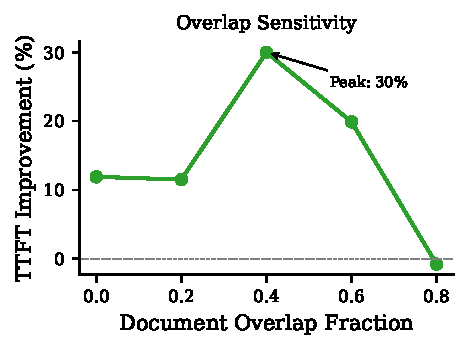
\includegraphics[width=0.85\linewidth]{figures/overlap_sensitivity.pdf}
\caption{TTFT improvement vs.\ \emph{nominal} overlap fraction (the parameter fed to the trace generator). Note: the $x$-axis is the generator parameter, not the actual Jaccard; the 0.0 and 0.2 points both produce an actual Jaccard of $\approx$0.39 due to the generator's minimum-sharing floor (see Section~\ref{sec:eval} and Table~\ref{tab:overlap_raw}).}
\label{fig:overlap}
\vspace{-1em}
\end{figure}

This result is useful because it clarifies the operating regime of the method. RAGCache++ is not a universal speedup for all workloads. It is most effective when requests are related enough to share evidence, but not so similar that the retriever already returns the same order.


\subsection{Answer Quality Preservation}

A natural concern is whether document reordering changes what the model answers. On our extractive QA setting, the answer does not change. This is consistent with the design of the method: we reorder evidence, but we do not remove any retrieved content.

\textbf{Interpretation.} For tasks where the answer is explicitly present in the retrieved passages, evidence order is usually less important than evidence availability. In this regime, reordering mainly changes prefill cost, not task information.

\paragraph{Multi-hop reasoning.}
\label{sec:multihop}

We also test a small multi-hop setting, where the answer requires combining two pieces of evidence. Here the absolute difficulty depends on the evidence arrangement itself, but within each evidence arrangement, optimized ordering and retrieval ordering give the same quality.

\begin{table}[t]
\caption{Multi-hop reasoning: does ordering disrupt evidence chains? (Qwen2.5-7B, 40 two-hop QA pairs, 3 distractors each.)}
\label{tab:multihop}
\centering
\small
\begin{tabular}{@{}llccc@{}}
\toprule
\textbf{Evidence} & \textbf{Doc Order} & \textbf{EM} & \textbf{Contains EM} & \textbf{F1} \\
\midrule
Natural   & Retrieval  & 0.675 & 0.775 & 0.862 \\
Natural   & Optimized  & 0.675 & 0.775 & 0.862 \\
Reversed  & Retrieval  & 0.625 & 0.750 & 0.826 \\
Reversed  & Optimized  & 0.625 & 0.750 & 0.826 \\
\bottomrule
\end{tabular}
\vspace{-0.5em}
\end{table}

This result is reassuring but should be interpreted carefully. It does not prove that order never matters for reasoning. It shows a narrower claim: in our test suite, the ordering policy did not introduce an observable quality drop.


\subsection{Systems Analysis}
\label{sec:systems}

The rest of this section asks whether the TTFT gains come with hidden systems costs. Our answer is largely no.

\paragraph{Latency profiling.}
Table~\ref{tab:profiling} separates ordering, prompt construction, and model execution. The main message is simple: the added CPU-side work is tiny, while the inference stage becomes noticeably faster because more prefix blocks can be reused.

\begin{table}[t]
\caption{Per-request latency breakdown (RTX 4090, 195 post-warmup queries). APC+Opt.\ Order+Build totals 66\,$\mu$s (incremental ${\sim}$26\,$\mu$s over APC+Retr.) while reducing inference p50 by 29\%.}
\label{tab:profiling}
\centering
\small
\resizebox{\columnwidth}{!}{%
\begin{tabular}{@{}lccccc@{}}
\toprule
\textbf{Strategy} & \textbf{Order} & \textbf{Build} & \textbf{Gen.\ (mean)} & \textbf{Gen.\ (p50)} & \textbf{OH} \\
\midrule
APC+Retr. & 4.0\,$\mu$s & 36.3\,$\mu$s & 55.5\,ms & 58.6\,ms & 0.07\% \\
APC+Opt.  & 22.2\,$\mu$s & 44.4\,$\mu$s & 52.5\,ms & 41.4\,ms & 0.13\% \\
\bottomrule
\end{tabular}%
}
\vspace{-0.5em}
\end{table}

\paragraph{Throughput.}
For long-output workloads, decode dominates total time, so TTFT savings do not automatically translate into large throughput changes. Even so, optimized ordering matches baseline APC throughput closely, which means the method does not buy latency by quietly hurting overall serving capacity.

\begin{table}[t]
\caption{Throughput on RTX 4090 (Qwen2.5-7B, 200 queries, 50 output tokens each). tok/s counts total tokens processed (input prompt + output); e.g., sequential 1.19 req/s $\times$ ${\sim}$1{,}150 tokens/req $\approx$ 1{,}370 tok/s. Ordering matches baseline APC throughput ($<$0.4\% difference).}
\label{tab:throughput}
\centering
\small
\begin{tabular}{@{}lcccc@{}}
\toprule
 & \multicolumn{2}{c}{\textbf{Sequential}} & \multicolumn{2}{c}{\textbf{Batched}} \\
\cmidrule(lr){2-3}\cmidrule(lr){4-5}
\textbf{Strategy} & \textbf{req/s} & \textbf{tok/s} & \textbf{req/s} & \textbf{tok/s} \\
\midrule
No Cache      & 1.10 & 1{,}270 & 7.88 & 9{,}064 \\
APC+Retrieval & 1.19 & 1{,}370 & 82.05 & 94{,}382 \\
APC+Optimized & 1.19 & 1{,}371 & 81.75 & 94{,}029 \\
\bottomrule
\end{tabular}
\vspace{-0.5em}
\end{table}

\paragraph{GPU memory.} We do not observe a meaningful GPU-memory penalty from ordering itself. This is expected, because the method changes reuse patterns inside the existing APC pool rather than increasing the pool size. The knowledge tree lives in host memory and is small in our experiments.

\paragraph{Pipelining analysis.}
The warmup-based pipelining design from Section~\ref{sec:design} behaves as expected in end-to-end measurements. When retrieval is not negligible, overlapping retrieval with reusable system-prompt prefill produces additional savings.

\begin{table}[t]
\caption{End-to-end pipelining: measured wall-clock TTFT (RTX 4090). Serial $=T_{\text{ret}}+T_{\text{cold}}$ with $T_{\text{cold}}=56.8$\,ms; Pipelined $=\max(T_{\text{ret}},T_{\text{sys}})+T_{\text{warm}}$ with $T_{\text{sys}}=21.6$\,ms and $T_{\text{warm}}=28.2$\,ms.}
\label{tab:pipelining_e2e}
\centering
\small
\begin{tabular}{@{}cccr@{}}
\toprule
\textbf{$T_{\text{ret}}$ (ms)} & \textbf{Serial (ms)} & \textbf{Pipelined (ms)} & \textbf{Saving} \\
\midrule
20  & 76.8  & 50.4  & 34.4\% \\
50  & 106.8 & 78.8  & 26.2\% \\
100 & 156.8 & 128.8 & 17.9\% \\
\bottomrule
\end{tabular}
\vspace{-0.5em}
\end{table}

\paragraph{Cache efficiency.}
The cache-efficiency analysis is consistent with the TTFT results. Optimized ordering not only creates reuse more often, but more importantly, creates reuse of greater depth.

\begin{table}[t]
\caption{Cache efficiency: prefill saved per request (RTX 4090, 195 queries, No-Cache p50 = 116\,ms in this run; differs from Table~\ref{tab:main}/\ref{tab:baselines} due to independent benchmark runs per Section~\ref{sec:eval}).}
\label{tab:cache_eff}
\centering
\small
\resizebox{\columnwidth}{!}{%
\begin{tabular}{@{}lcccc@{}}
\toprule
\textbf{Strategy} & \textbf{Saved (p50)} & \textbf{Saved (mean)} & \textbf{Saved (p95)} & \textbf{Benefit} \\
\midrule
APC+Retr. & 50.1\% & 52.8\% & 75.6\% & 176/195 \\
APC+Opt.  & 66.3\% & 57.6\% & 77.7\% & 185/195 \\
\bottomrule
\end{tabular}%
}
\vspace{-0.5em}
\end{table}

\paragraph{Concurrent load.}
The gains also survive under concurrent execution. This matters because sequential traces can sometimes overstate locality. In our batched experiments, the improvement becomes smaller than in the single-request case, but it remains visible across all tested batch sizes.

\begin{table}[t]
\caption{Concurrent load: avg per-request TTFT at different batch sizes (RTX 4090, 200 queries). Ordering benefit persists across all concurrency levels.}
\label{tab:concurrent}
\centering
\small
\begin{tabular}{@{}ccccr@{}}
\toprule
\textbf{Batch} & \textbf{No Cache} & \textbf{APC+Retr.} & \textbf{APC+Opt.} & \textbf{Improv.} \\
\midrule
1 & 114.7 & 54.7 & 50.7 & 7.3\% \\
2 & 110.5 & 48.0 & 44.3 & 7.7\% \\
4 & 103.4 & 41.6 & 37.5 & 9.9\% \\
8 & 100.9 & 38.3 & 35.7 & 6.8\% \\
\bottomrule
\end{tabular}
\vspace{-0.5em}
\end{table}

\paragraph{Baseline comparison.}
We compare the greedy walk with several alternative orderings, including a recency heuristic and an exhaustive oracle. The greedy method is already very close to oracle, which suggests that expensive search is unnecessary for this problem size.

\begin{table}[t]
\caption{Ordering baselines (RTX 4090, 195 queries). All six strategies measured in a single consistent run with one shared trace. Greedy trie achieves 97.5\% of oracle's TTFT reduction (+29.6\% vs.\ oracle's +30.3\%).}
\label{tab:baselines}
\centering
\small
\resizebox{\columnwidth}{!}{%
\begin{tabular}{@{}lccr@{}}
\toprule
\textbf{Strategy} & \textbf{p50 (ms)} & \textbf{Mean (ms)} & \textbf{vs.\ Retr.} \\
\midrule
No Cache & 121.55 & 121.73 & -- \\
APC+Sorted & 81.75 & 77.42 & $-35.5$\% \\
APC+Retrieval & 60.34 & 57.63 & baseline \\
APC+Recency & 59.52 & 56.62 & $+1.4$\% \\
APC+Optimized (Ours) & \textbf{42.50} & \textbf{53.77} & $+29.6$\% \\
APC+Oracle & 42.04 & 53.08 & $+30.3$\% \\
\bottomrule
\end{tabular}%
}
\vspace{-0.5em}
\end{table}

\paragraph{Robustness.} Additional sweeps over cache pressure and context length show that the improvement is not tied to one narrow memory setting. The exact percentage changes from run to run, but the qualitative result remains stable.

\paragraph{Generality.} We also test models outside one scale point and find that the benefit is not unique to a single model size. The magnitude changes, but the same ordering effect appears across the tested configurations.

\paragraph{Geospatial workload.}
\label{sec:spatial}

To move beyond the main synthetic benchmark, we construct a geospatial workload inspired by Spatial-RAG and ItiNera~\citep{yu2025spatialrag,tang2024itinera}. The overlap in this workload is lower and less controlled, so it is a useful stress test for whether the method still helps when reuse opportunities are weaker and more irregular.

\begin{table}[t]
\caption{Geospatial workload results (RTX 4090, 200 queries, avg Jaccard = 0.17).}
\label{tab:spatial}
\centering
\small
\begin{tabular}{@{}lccc@{}}
\toprule
\textbf{Strategy} & \textbf{p50 (ms)} & \textbf{p95 (ms)} & \textbf{Mean (ms)} \\
\midrule
No Cache      & 110.3 & 113.1 & 109.5 \\
APC+Retrieval & 96.5  & 103.1 & 96.1  \\
APC+Optimized & \textbf{92.2} & \textbf{103.0} & \textbf{85.7} \\
\bottomrule
\end{tabular}
\vspace{-0.5em}
\end{table}

The gain is smaller here than in the bursty synthetic benchmark, which is exactly what we would expect from the lower overlap level. Even so, the direction is still positive, showing that the method does not rely on one artificial trace shape.


\subsection{Workload Diversity}
\label{sec:nq}

We further evaluate three workloads with different overlap regimes. The goal is not to claim one universal number, but to show how the benefit changes with workload structure.

\paragraph{NQ-Open (high overlap, Jaccard = 0.88).}
\label{sec:nq_open}
Using a corpus derived from Natural Questions~\citep{kwiatkowski2019nq}, we obtain a very high-overlap trace. In this setting, APC in retrieval order is already strong, so our extra gain is small. This is consistent with the overlap-sensitivity result above.

\paragraph{Mixed-topic (moderate overlap, Jaccard = 0.31).}
With a trace that alternates between related and unrelated topics, the benefit becomes more visible again. This is the regime where ordering feels most natural: there is enough repeated evidence to exploit, but enough variation that retrieval order is no longer cache-friendly.

\paragraph{Wikipedia-style TF-IDF (low natural overlap, Jaccard = 0.06).}
\label{sec:real_corpus}
Finally, we build a larger, more diverse corpus and use TF-IDF retrieval without manually controlling overlap. Even though the mean overlap is low, optimized ordering still helps, suggesting that temporal locality inside the trace matters more than a single global Jaccard number.

\begin{table}[t]
\caption{Wikipedia-style corpus evaluation with TF-IDF retrieval (RTX 4090, 200 queries, 1{,}000 constructed passages / 20 topics; mean Jaccard = 0.06, no controlled overlap).}
\label{tab:real_corpus}
\centering
\small
\resizebox{\columnwidth}{!}{%
\begin{tabular}{@{}lcccc@{}}
\toprule
\textbf{Strategy} & \textbf{p50 (ms)} & \textbf{p95 (ms)} & \textbf{Mean (ms)} & \textbf{vs.\ Retr.} \\
\midrule
No Cache      & 45.8 & 54.1 & 47.2 & -- \\
APC+Retrieval & 33.9 & 46.8 & 34.2 & baseline \\
APC+Optimized & \textbf{24.8} & \textbf{46.5} & \textbf{27.2} & +26.8\% \\
\bottomrule
\end{tabular}%
}
\vspace{-0.5em}
\end{table}


\subsection{End-to-End Pipeline Latency}
\label{sec:e2e}

In deployment, retrieval latency comes before inference. Table~\ref{tab:e2e} therefore reports end-to-end TTFT with simulated retrieval delay. The improvement becomes smaller once retrieval takes a larger share of total time, but it remains visible, especially at lower batch sizes where prefill cost is less amortized.

\begin{table}[t]
\caption{End-to-end TTFT (ms) including retrieval latency (RTX 4090, 200 queries; workload generates 50 output tokens per request but TTFT excludes the 50-token decode).}
\label{tab:e2e}
\centering
\small
\begin{tabular}{@{}ccccr@{}}
\toprule
$T_{\text{ret}}$ & \textbf{Batch} & \textbf{APC+Retr.} & \textbf{APC+Opt.} & \textbf{Improv.} \\
\midrule
\multirow{3}{*}{10\,ms} & 1 & 69.6 & 51.8 & 25.6\% \\
 & 4 & 51.8 & 46.9 & 9.5\% \\
 & 8 & 48.9 & 45.9 & 6.1\% \\
\midrule
\multirow{3}{*}{30\,ms} & 1 & 89.7 & 72.4 & 19.3\% \\
 & 4 & 71.8 & 67.8 & 5.6\% \\
 & 8 & 68.8 & 66.8 & 2.9\% \\
\midrule
\multirow{3}{*}{50\,ms} & 1 & 109.3 & 92.2 & 15.6\% \\
 & 4 & 91.8 & 87.4 & 4.8\% \\
 & 8 & 88.7 & 86.3 & 2.7\% \\
\bottomrule
\end{tabular}%
\vspace{-0.5em}
\end{table}


\subsection{System Validation}
\label{sec:trie_valid}

Our method relies on the trie as an approximation of real APC state, so we also check whether this approximation is reasonable. The observed correlation between predicted reuse and TTFT-implied reuse is high, which supports the basic design choice.

\paragraph{Integrated pipeline.}
\label{sec:integrated}

When we evaluate the full proxy with feedback and pruning, the overall behavior remains close to the simpler ordering wrapper. In other words, the extra bookkeeping does not remove the benefit that motivates the method in the first place.



\section{Conclusion and Discussion}
\label{sec:conclusion}
% ================================================================

We presented RAGCache++, a prompt-layer method for improving KV reuse in APC-based RAG serving. The main idea is to reorder retrieved documents so that the final prompt is more likely to match a recently cached prefix. This design is intentionally small. It does not require changes to the serving engine, and it still delivers consistent TTFT gains across our main benchmarks.

The main takeaway is straightforward. In APC-based RAG, cache efficiency is not decided only by the model or the serving backend. It is also shaped by how retrieved evidence is arranged before inference. From this perspective, document ordering is a lightweight scheduling problem between retrieval and serving. Our experiments show that even a simple greedy trie walk is already enough to recover much of the lost locality. The method stays close to oracle ordering, adds very little CPU overhead, and does not hurt answer quality in our QA tests.

At the same time, the method has clear limits. It works best when the workload has some temporal locality and moderate document overlap. If overlap is already extremely high, retrieval order is often good enough. If overlap is truly low, there is little reusable structure to exploit. Our evaluation is also still limited in scale. We do not test large multi-tenant traces or production traffic, and we only study a small set of models and retrieval settings.

There are several natural directions for future work. One is to combine prompt-layer ordering with position-insensitive reuse methods, so that both prefix-compatible and non-prefix-compatible sharing can be exploited. Another is to use more direct cache-state signals from the engine when they are available, instead of relying mainly on the trie as an approximation. A third is to evaluate the method on more realistic traces where locality comes from user behavior rather than from controlled synthetic bursts. Overall, we view this work as a practical systems result: before redesigning the cache itself, it is already worth asking whether the prompt can be arranged in a more cache-friendly way.

\section{Team Member Contributions}
\label{sec:contrib}

\begingroup
\sloppy
\emergencystretch=3em

\paragraph{Kaizhen Tan.}
Led the overall project design, the main system implementation, and most of the paper writing. He was primarily responsible for the prompt-layer reordering pipeline and its integration with the vLLM serving path, including the core prompt construction and request handling logic. He also ran most of the main latency experiments, including the TTFT comparison and the end-to-end evaluation, and took the lead in revising the abstract, introduction, methodology, and experiments sections.

\paragraph{Rong Gu.}
Contributed to the cache-side implementation and system validation. He worked on the main cache data structures and management logic, including the knowledge-tree organization and cache bookkeeping modules. He also helped with profiling, cache-efficiency analysis, and revision of the implementation and discussion sections.

\paragraph{Mingyuan Li.}
Contributed to workload construction, experimental evaluation, and result analysis. He helped build the QA-based and workload-diversity experiments, including the overlap-sensitivity and multi-domain settings, and assisted with result checking and revision of the analysis, findings, and conclusion sections.

\endgroup

\appendix

\section{Experimental Configuration Details}
\label{app:config}

This appendix lists the hardware and software settings used in the main experiments.

\begin{table}[H]
\caption{Hardware and software configuration.}
\centering
\footnotesize
\begin{tabular}{@{}lll@{}}
\toprule
 & \textbf{Config A} & \textbf{Config B} \\
\midrule
GPU & 4060\,Ti 8\,GB & 4090 24\,GB \\
Model & Qwen2.5-1.5B & Qwen2.5-7B \\
vLLM & 0.8.5.post1 & 0.17.1 \\
\texttt{max\_model\_len} & 2048 & 4096 \\
\texttt{gpu\_mem\_util} & 0.85 & 0.90 \\
Corpus & 100 docs & 500 docs \\
Queries & 100 & 200 \\
Top-$k$ & 5 & 5 \\
Use & TTFT, overlap & All (\S\ref{sec:eval}--\ref{sec:trie_valid}) \\
\bottomrule
\end{tabular}%

\end{table}


\section{Overlap Sweep Raw Data}
\label{app:overlap}

This appendix reports the raw numbers behind the overlap-sensitivity figure in the main text.

\begin{table}[H]
\caption{Raw data for overlap sensitivity (RTX 4060~Ti, Qwen2.5-1.5B-Instruct).}
\label{tab:overlap_raw}
\centering
\footnotesize
\begin{tabular}{@{}ccccc@{}}
\toprule
\textbf{Overlap} & \textbf{Jaccard} & \textbf{Retrieval} & \textbf{Optimized} & \textbf{Improv.} \\
\textbf{Frac.} & & \textbf{p50 (ms)} & \textbf{p50 (ms)} & \\
\midrule
0.0 & 0.386 & 126.8 & 111.7 & 11.9\% \\
0.2 & 0.386 & 128.9 & 114.2 & 11.5\% \\
0.4 & 0.417 & 111.1 & 77.8  & 30.0\% \\
0.6 & 0.526 & 75.5  & 60.5  & 19.9\% \\
0.8 & 0.661 & 50.4  & 50.8  & $-0.8$\% \\
\bottomrule
\end{tabular}
\end{table}


\section{Systems Benchmark Details}
\label{app:v100}

The systems analysis in Section~\ref{sec:systems} uses Config~B (RTX 4090) with \texttt{enforce\_eager=True}, so CUDA graphs are disabled for more stable measurement.

\bibliography{references}
\bibliographystyle{mlsys2024}

\end{document}
